% !TeX root = ../dlmu.tex


\section{绪论}
\subsection{无人驾驶及路径规划相关背景}
随着世界经济的腾飞,机动车数量迅速增长。其不可避免的带来了环境与交通事故,
据统计,交通事故是导致现代人非自然死亡的最主要原因,于是研究人员提出可以使用车辆智能化技术即无人驾驶来解决这些难题。目前,无人驾驶已是各国研究的重点,其在缓解交通拥堵,改善空气质
量,提高出行安全方面有着重大意义。各国目前也在无人驾驶领域,给予了企业很多政策和经济上的便利。

据目前通用的业内标准\upcite{r1},无人驾驶有L0\~{}L5六个级别。如表~\ref{tab:tab1}所示,其中L3以上级别,由驾驶设备观测环境,完成汽车加减速等大部分驾驶动作。无人驾驶每个级别的突破都具有极大难度,尤其是L4到L5。目前各个企业研究的重点也都是在L4范围内的自动驾驶。
\begin{table}[H]
  \centering
  \caption{ \textbf{自动驾驶分级标准\upcite{r1}}}
  \begin{tabular}{lc}
    \toprule
    级别          &       自动化程度                         \\
    \midrule
    L0   & 完全由人类驾驶\\
    L1   & 驾驶设备完成小部分驾驶动作,仅适应限定区域                     \\
    L2 & 驾驶设备完成一部分驾驶动作,仅适应限定区域    \\
    L3 & 驾驶设备完成大部分驾驶动作,仅适应限定区域  \\
    L4 & 驾驶设备完成所有驾驶动作,仅适应限定区域        \\
    L5 & 驾驶设备完成所有驾驶动作,适应于各种区域       \\
    \bottomrule
  \end{tabular}
  \label{tab:tab1}
\end{table}

无人驾驶是一项复杂的技术,它包含了许多前沿的研究领域,其通过不同领域技术的融合,在无人控制
或部分人为干预的情况下,将货物或乘客运送到目的地。具体的,无人驾驶研究领域包含感知、决策、运动控制等多个模块。

Perception(感知)是指利用高精度地图信息与传感器数据,经过计算与处理后,对车辆周围的环境来进行感知。
但是无人驾驶不能过度依赖于感知模块,否则一旦感知模块失灵,无人驾驶的安全性便没了保证。
自动驾驶系统需要做到即使在某些模块故障的情况下也能做出稳妥的
行为,安全的完成任务。

自动驾驶的决策通常是指根据感知预测模块输入的信息,控制汽车驾驶行为以达到驾驶目标。
因此决策模块需要至少包括两方面即长期路径规划以及局部路径规划,由此可以说路径规划是无人驾驶决策的核心组成部分。
长期路径规划也称为全局路径规划一般选取A*算法或者Dijkstra,D*等基于搜索的算法,
局部路径规划也称短期路径规划,常用的有DWA、人工势场法等。这些全局规划算法大都可以规划出
一条无碰的路径以完成行车目标,但这些方法没有充分考虑到人的驾驶习惯,即有的人可能喜欢走大道,
有的人可能喜欢走观光通道,有时候路径规划的首要考虑因素是快速到达,有时路径规划 可能
是为了更好的欣赏美景,这些基于不同场景不同需求的路径规划,传统算法无法进行很好的解决。
哪怕使用规则进行不同场景的描述,也无法枚举到所有情况,得到令人满意的结果。

\subsection{国内外相关研究现状}

\subsubsection{无人驾驶决策国内外研究现状}
目前,无人驾驶的决策方法大致可分为基于规则的方法和基于强化学习或深度学习的方法。
作为无人驾驶的决策模块,其需要在保证安全的前提下,完成人类交给车辆的各种任务。
下面将分别介绍三家知名无人驾驶技术公司的技术路线。
Mobileye使用传感器以及云端地图,再加上独立的决策模块以实现无人驾驶。
值得
提及的是Mobileye公司最初是做计算机视觉的公司,后来开始从事无人驾驶相关研究,其将深度学习算法与计算机视觉算法结合起来,已经可以做到
仅用摄像机,做到一定范围内安全舒适的无人驾驶体验,体现了其在感知模块的强大实力,在决策模块Mobileye公司使用深度强化学习作为决策模块,
将目标划分为可学习部分与不可学习部分,在确保安全的同时也使系统鲁棒性上升。
\begin{figure}[htbp]
\centering
\subfigure[Apollo]{
\begin{minipage}[t]{0.33\linewidth}
\centering
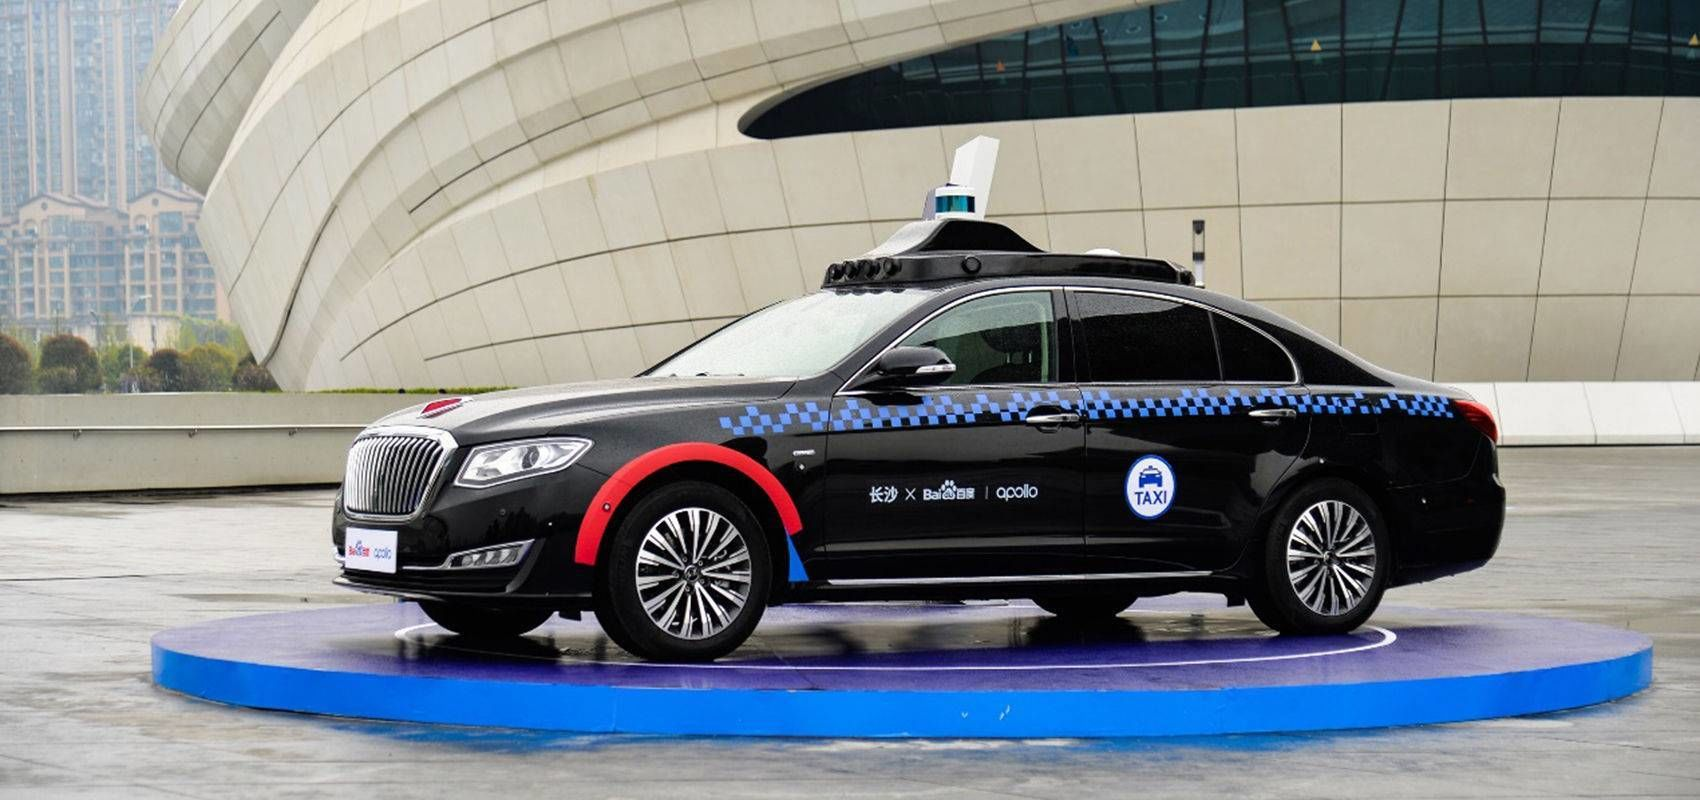
\includegraphics[width=4cm,height=3cm]{fig/apollo.jpg}
%\caption{fig1}
\end{minipage}%
}%
\subfigure[Mobileye]{
\begin{minipage}[t]{0.33\linewidth}
\centering
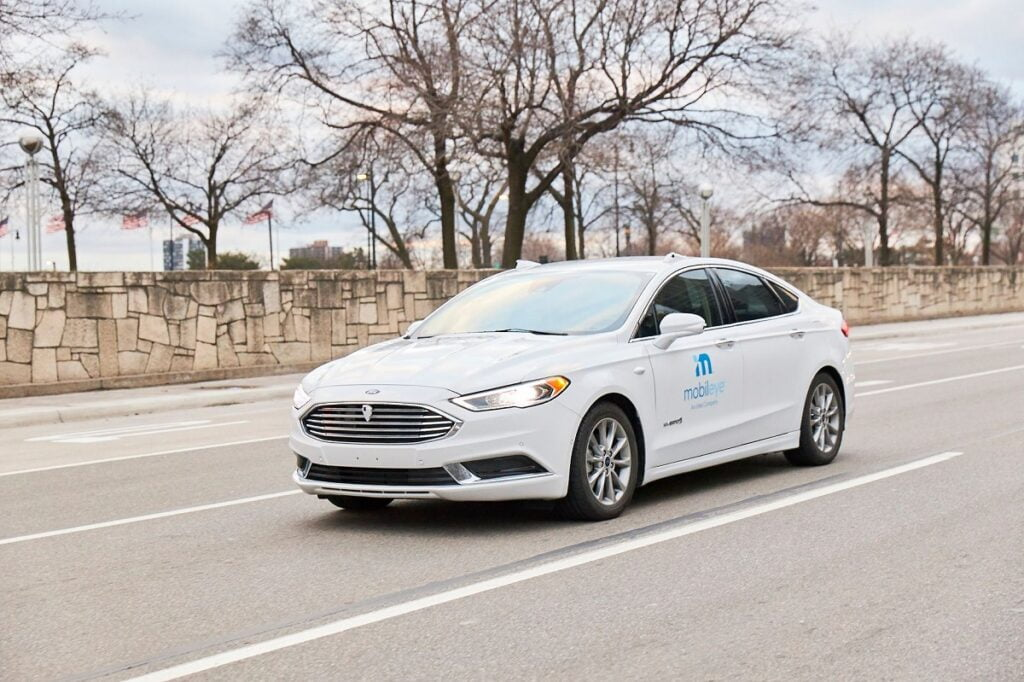
\includegraphics[width=4cm,height=3cm]{fig/mobileye.png}
%\caption{fig2}
\end{minipage}%
}%
\subfigure[Waymo]{
\begin{minipage}[t]{0.33\linewidth}
\centering
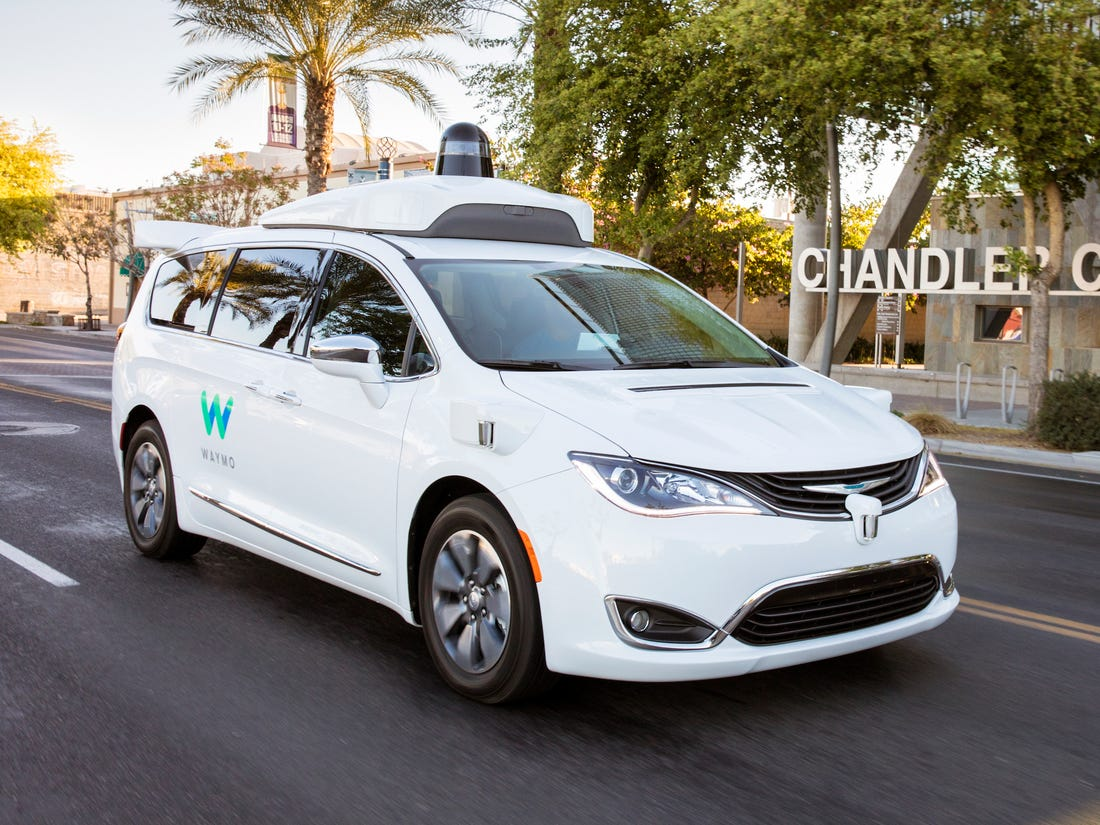
\includegraphics[width=4cm,height=3cm]{fig/waymo.jpg}
%\caption{fig2}
\end{minipage}
}%
\centering
\caption{ \textbf{无人驾驶车辆}}
\end{figure}

百度的Apollo项目特点在于其决策依赖于大量周围环境的信息,包括但不限于行人、车道线等。
在Apollo中,决策层和运动控制层有一个被称为优化层的模块,其主要作用是隔离决策层与上层模块,以减少对环境信息的依赖。虽然
Apollo已实现实用场合下的自动驾驶,例如百度在长沙进行的无人驾驶出租车测试,并已开始批量生产
无人驾驶车辆,
但是百度基于场景设计的决策模块需要与诸如智能公路这样的基础设施相结合,才能发挥出最佳效果,这点就需要与我国
优秀的基建能力相结合。

Google开发的Waymo,其特点是利用仿真器训练车辆,使其成为一个优秀的"驾驶员"。
Waymo使用自制的仿真器,其可以模拟车辆运行时的真实情况且可以创造特殊场景以供智能车训练。
。Waymo基本的技术路线是实现单车智能,即车辆的无人驾驶并不依赖于周围人造的基础设施。
Waymo遵循感知-预测-决策的系统框架。
决策组件输入感测和预测信息,并同时在设计和操作范围内
进行安全行驶。此外,Waymo的决策模块也融入了深度强化学习算法。


\subsubsection{路径规划研究现状}
路径规划广义上可划分为两种,即全局和局部。全局路径规划指在起始点和终止点之间规划出无碰轨迹。
局部路径规划,主要是指将一个个导航点输出为速度指令。下面将分别进行叙述。

(1)全局路径规划算法

全局路径规划在已知地图信息的情况下,规划出从起始点到终止点的无碰路径。按照
研究方向可以大致分为智能算法\upcite{r2,r14,r15,r22}和传统算法\upcite{r16}。

1)传统算法

 Dijkstra\upcite{r12}算法于1959 年 被提出。该算法可以找到起始点到目标点的最短路径,但缺点是运算复杂度高。
美国曼彻斯特大学的 Holland JH 教授于1967 年通过模拟生物进化和遗传理论,提
出了遗传算法\upcite{r10}并用于路径规划中。该算法的问题是可能陷入局部最优解,虽然后来有过改进,但仍不理想
。
 Hart 等人于1968 年提出启发式算法Astar \upcite{r11}算法。其作为 Dijkstra 算法的改进,可以十分高效的进行路径规划
 ,Astar 算法也一跃成为最常用的路径规划算法之一,但Astar算法在面对大尺度地图时,规划时间过长,甚至失败。
后来,人们又提出了如RA*\upcite{r8}算法以用于大尺寸地图,之后各种类似的算法如D*算法,DLite算法也都是在A*算法的基础上进行改进,
在各自擅长的方面取得了不错的效果。

2)智能算法

智能算法主要是指将机器学习的方法用于路径规划中来。如强化学习中的Qlearning算法\upcite{r13},神经网络算法等。这些算法在路径规划
中使用时,对比传统的A*\upcite{r11}等启发式算法没有明显的优势。但如Qlearning之类的智能算法,大都实现的是端到端的学习。其不需要事先知道环境地图
而是通过与外界的交互,找出路径,这点就跟人类探索环境很像。

(2)局部路径规划算法

局部路径规划将全局路径规划输出的导航点转换成速度指令,并能躲避出现在两导航点之间的动态障碍物。
这里主要介绍DWA(动态窗口法)\upcite{r21}。

DWA算法,通过在动力学允许的范围内,采样多组速度,并模拟这些速度在的相应运动轨迹
,再评价这些轨迹,选取得分最高的最优路径,并把相应的速度控制指令发送给机器人。该算法的特点在于
依据移动机器人的动力学性能限定速度采样空间在一定范围内。DWA算法之所以能成为一个广泛应用的局部路径算法,是因为
它很好的考虑到了
车辆的运动学模型,并输出了速度控制指令以到达各个导航点。

\subsubsection{深度强化学习研究现状}
强化学习\upcite{r9},简称RL,它与机器学习的其他研究领域有一定的区别,强化学习不需要专家的样本来对动作进行指导,
这是它与监督学习的区别,与非监督学习的区别在于强化学习的目的并不在于找到无任何标记的数据的背后的隐含的关系,
强化学习大都有直接的目的,如下棋游戏获得胜利等。强化学习的目的是最大化环境给予的奖励。这个过程大都满足马尔科夫性质,所以RL可以利用此性质简化计算。RL天生的决策能力再加上神经网络的抽象表达能力结合而成的深度强化学习(Deep Reforcement Learning)简称DRL
被视为是一种很有可能实现终极AI的方案。深度强化学习
按是否依赖环境模型
, 可 分 为 有 模 型RL算 法
(Model-based RL)和无模 型RL算 法(
Model-free RL )
。 深度强化学习按优化对象来 分类 , 可
分 为 基于 值 ( Value Optimization ) 和 基 于 策 略 的 优化算法
(Policy Optimization )
。 基 于 值 的  算 法 以 状 态(
state value function )或 动 作(
state-action value function )  价值 函 数  为 优化 目 标 ,通过最大化二者之一获得最优策略。 基于 策 略的算法 则直接对策 略 进行
操作,以求获得最优策略 。 这两种算法各有利弊
。基于值的算法有,Goole团队用于Atari游戏的DQN算法,其作为深度强化学习的鼻祖,为后来的研究人员指明了方向。基于策略的
算法有A3C\upcite{r5}、TRPO\upcite{r4}等。两种算法之间也可以相互结合,产生如DDPG\upcite{r6}、SAC\upcite{r3}等结合二者之长的算法\upcite{r17}。
从近年来论文发表的数量上看\upcite{r23,r24,r25,r26,r27,r28},DRL将会掀起机器学习领域新的一轮研究热潮。

\subsection{本文研究内容及篇章结构}
本文针对无人驾驶决策中存在的问题,提出使用深度强化学习中的DQN(深度Q学习)方法
来实现一个端到端的决策模块,并在Carla\upcite{r18}仿真环境中进行了车道保持任务的测试。针对传统路径规划方式无法有效的考虑人的喜好来规划路径,采用基于强化学习
的方法来进行路径规划,强化学习通过与环境的交互获得奖励,根据奖励最大化原则来规划路径,
可以通过奖励函数的个性化设计来适应每个人的需求,从而达到以人为本的路径规划。针对无人驾驶
仿真成本大的问题,本文在Carla仿真平台下进行仿真,来验证方案是否有效。
本文一共四章,每个章节的安排如下:

第一章绪论对无人驾驶领域的研究意义和基本常识做了一定介绍,通过对无人驾驶的介绍引入了无人驾驶决策部分的路径规划模块,
从而引出了利用强化学习实现“以人为本”的路径规划。通过对不同车企无人驾驶研究路线的讲述,介绍了无人驾驶目前研究现状。介绍了深度强化学习的研究现状,最后叙述了本文研究内容,并简述每章概要。

第二章对本文涉及到的决策模块进行介绍,要想设计出好的决策模块需要对无人车系统的其他部分也要有一定了解。
所以第二章介绍了无人驾驶系统的感知、决策和运动控制模块。接着介绍了本文所用无人驾驶仿真环境Carla。

第三章介绍了本文所用的强化学习路径规划算法以及深度强化学习车道保持算法。从强化学习开始讲起,详细讲述了
强化学习的相关知识,简单介绍了神经网络的知识。说明了本文所用的强化学习路径规划算法的基本原理。对本文所用
的DQN车道保持算法进行了介绍。

第四章验证了本文提出的强化学习路径规划算法和深度强化学习车道保持算法,并对实验结果进行分析与总结。包括两个部分,第一部分为使用强化学习的路径规划
采用了SARSA算法以及Q学习算法来进行路径规划,并对路径规划效果进行了分析。第二部分采用Carla仿真环境
在地图Town3中测试了基于DQN的车道保持效果,主要介绍了训练数据的预处理过程以及车道保持实验结果。

结尾部分根据本文所作工作进行总结与展望。








